\chapter{Sopraelevazione}

Un altro grafico elaborato dal programma mostra come variano i valori di sopraelevazione, ovvero delle pendenze trasversali. Per creare una sopraelevazione, si sfrutta un template già preimpostato per categoria di strada: esso deve rispettare la tipologia di strada F extraurbana, per cui dal decreto ministeriale del 5/11/2001 si leggono i valori di larghezza minima della corsia e della banchina.

\begin{figure}[H]
	\centering
	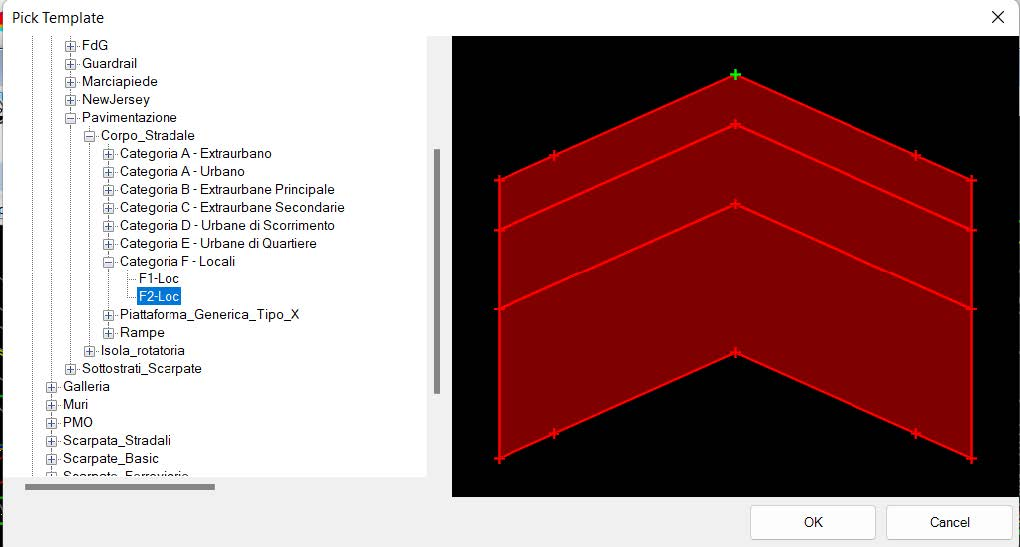
\includegraphics[width=\linewidth]{Figures/template}
	\captionof{figure}{template}
    \label{fig:template}
\end{figure}

Utilizzando il comando Create Superelevation Section nella sezione Corridors/Superelevation si creerà la sopraelevazione che sarà visibile sul tracciato planimetrico.

\begin{figure}[H]
	\centering
	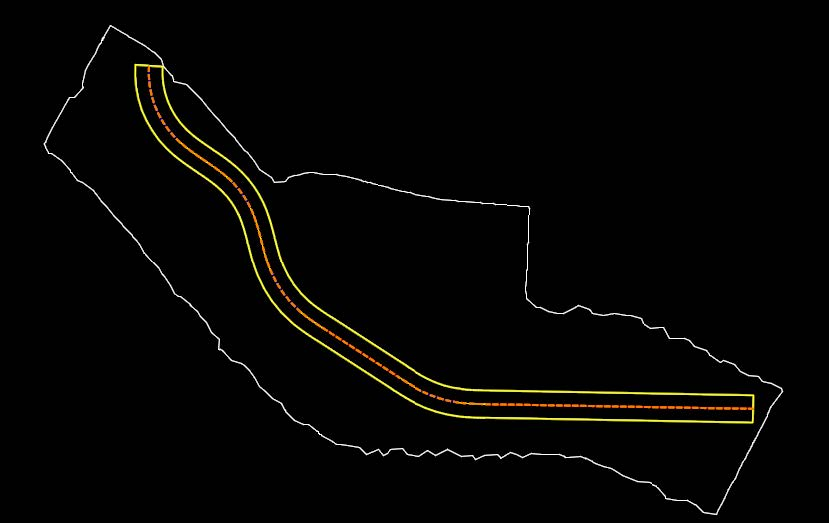
\includegraphics[width=\linewidth]{Figures/Sopraelevazione del tracciato vista in pianta}
	\captionof{figure}{Sopraelevazione del tracciato vista in pianta}
    \label{fig:Sopraelevazione del tracciato vista in pianta}
\end{figure}

Utilizzando ora il comando Calculate Superelevation il programma produrrà il profilo dei cigli del nostro tracciato.

\begin{figure}[H]
	\centering
	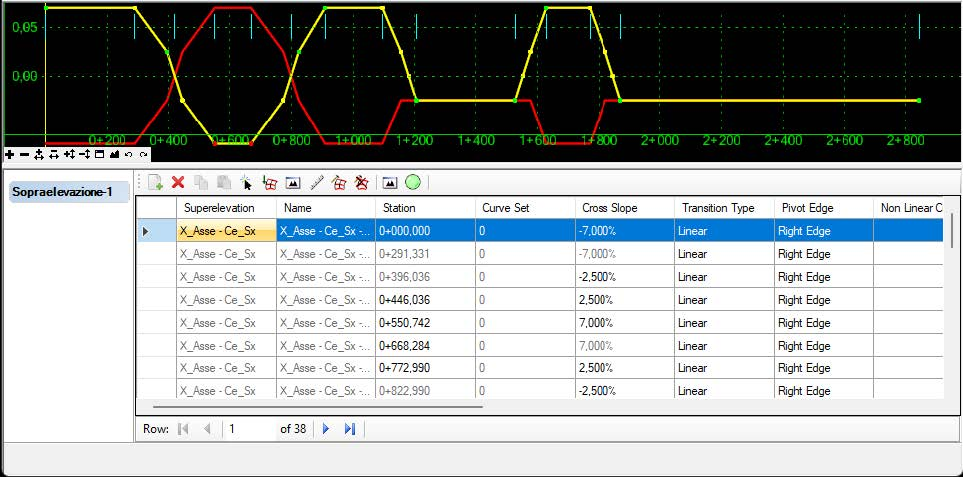
\includegraphics[width=\linewidth]{Figures/Profilo dei cigli}
	\captionof{figure}{Profilo dei cigli}
    \label{fig:Profilo dei cigli}
\end{figure}